\documentclass{article}
\usepackage{tikz}
\usepackage[margin=1in]{geometry} % full-width
\usepackage{graphicx}

% AMS Packages
\usepackage{amsmath}
\usepackage{amsthm}
\usepackage{amssymb}

% Unicode
\usepackage[utf8]{inputenc}


\usetikzlibrary{arrows.meta}
\newcommand {\axes}[4] {\draw[->] (0,0) -- (#3,0) node [right]{#1};\draw[->] (0,0) -- (0,#4) node[above]{#2};}
\newcommand {\valx}[2] {\draw (#1,0.03) -- (#1,-0.03) node[anchor=north]{#2};}
\newcommand {\valy}[2] {\draw (0.03,#1) -- (-0.03,#1) node[anchor=east]{#2};}

\title{TIPE Sur l'optimisation du traffic routier.}
\author{MOULAT Mathéo\\NODET Gaëtan\\DURAND Ulysse\\MARGUET Emeric}
\everymath{\displaystyle}
\date{\today}
\begin{document}

\maketitle

\section{Abstract}
Notre but est de proposer un outil de fluidification du traffic routier en supposant que l'on peut imposer un chemin à suivre à chaque véhicule. 


\section{Modèle 1} 

Le réseau routier sera un graphe où les sommets sont des croisements et les arrêtes des portions de route.\\
Le graphe est orienté et une route à double sens est représentée par deux arrêtes distinctes.\\
Les voitures vont toutes d'un sommet A du graphe à un autre sommet B.\\
Pour une voiture, le temps de parcours d'un croisement  est nul.
\\
Le régime est permanent, c'est à dire qu'on considère un nombre fixe de voitures présentes a chaque instant sur le graphe.\\
Un ensemble des voitures sera modélisé par un flux (on pourra donc parler de \textit{4,3} voitures sur la portion de route entre les sommets X et Y), ce nombre sera alors constant au cours du temps.\\
L'objectif est de minimiser le temps de parcours maximal.\\
Chaque segment a comme attribut une fonction qui au nombre de voiture sur le segment associe leur vitesse.
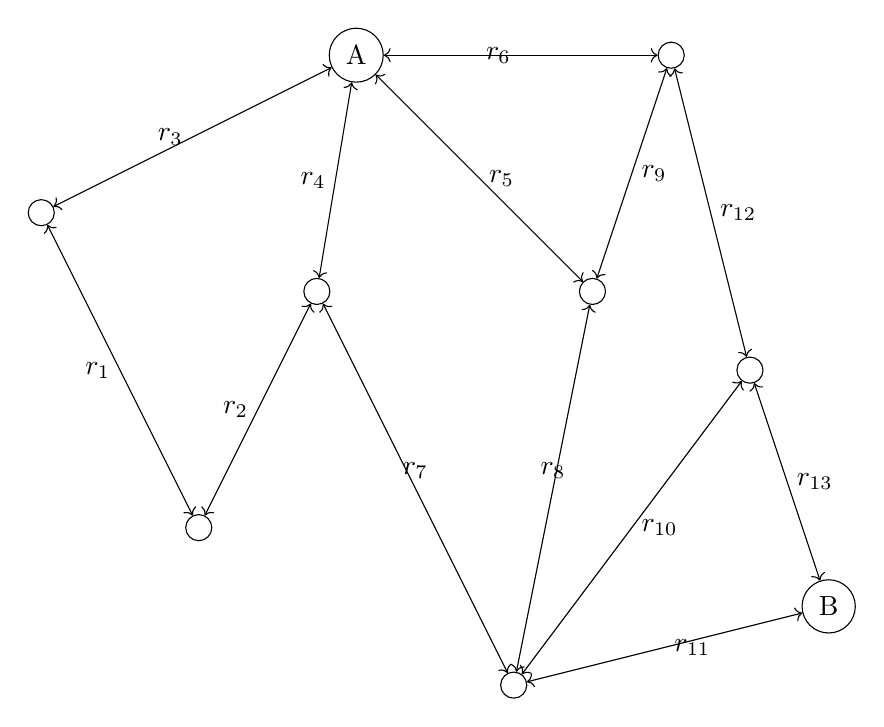
\begin{tikzpicture}
    \node[shape=circle,draw=black] (A) at (3,3) {};
    \node[shape=circle,draw=black] (B) at (1,7) {};
    \node[shape=circle,draw=black] (C) at (5,9) {A};
    \node[shape=circle,draw=black] (D) at (4.5,6) {};
    \node[shape=circle,draw=black] (E) at (7,1) {};
    \node[shape=circle,draw=black] (F) at (8,6) {} ;
    \node[shape=circle,draw=black] (G) at (9,9) {} ;
    \node[shape=circle,draw=black] (H) at (10,5) {} ;
    \node[shape=circle,draw=black] (I) at (11,2) {B} ;

    \path [<->] (A) edge node[left] {$r_1$} (B);
    \path [<->](A) edge node[left] {$r_2$} (D);
    \path [<->](B) edge node[left] {$r_3$} (C);
    \path [<->](C) edge node[left] {$r_4$} (D);
    \path [<->](C) edge node[right] {$r_5$} (F);
    \path [<->](C) edge node[left] {$r_6$} (G);
    \path [<->](D) edge node[above] {$r_7$} (E);
    \path [<->](F) edge node[above] {$r_8$} (E);
    \path [<->](F) edge node[right] {$r_9$} (G);
    \path [<->](E) edge node[right] {$r_{10}$} (H);  
    \path [<->](E) edge node[right] {$r_{11}$} (I);
    \path [<->](G) edge node[right] {$r_{12}$} (H);
    \path [<->](H) edge node[right] {$r_{13}$} (I);
\end{tikzpicture}
\newpage
\subsection{Modeles}
\subsubsection{}
\begin{tikzpicture}[scale=3]
    \axes{n}{v}{1}{0.6}
    \valx{0.9}{$n_{max}$}
    \valy{0.5}{$v_{max}$}
    \draw[{}-{Arc Barb [reversed]},line width = 0.3mm, color=red] (0,0.5) -- (0.9,0.5);
\end{tikzpicture}

Ce modèle très simpliste considère que les voitures roulent a vitesse constante ($v_{max}$) jusqu’à un nombre maximum de voitures pouvant utiliser la route en même temps ($n_{max}$). Peu réaliste, il prend tout de même en compte qu’une route ne peut pas accueillir un nombre illimité de voitures. De plus, il permet une implémentation relativement simple de l’algorithme de résolution.
\\\\
\paragraph {Algorithme de résolution : }
On utilisera l'algorithme de Dijkstra l\'egerement modifi\'e.\\
But de l'algorithme de Dijkstra : r\'esoudre le probl\`eme de plus court chemin. Ce probl\`eme est de trouver le plus court chemin dans un graphe pond\'er\'e orient\'e. \\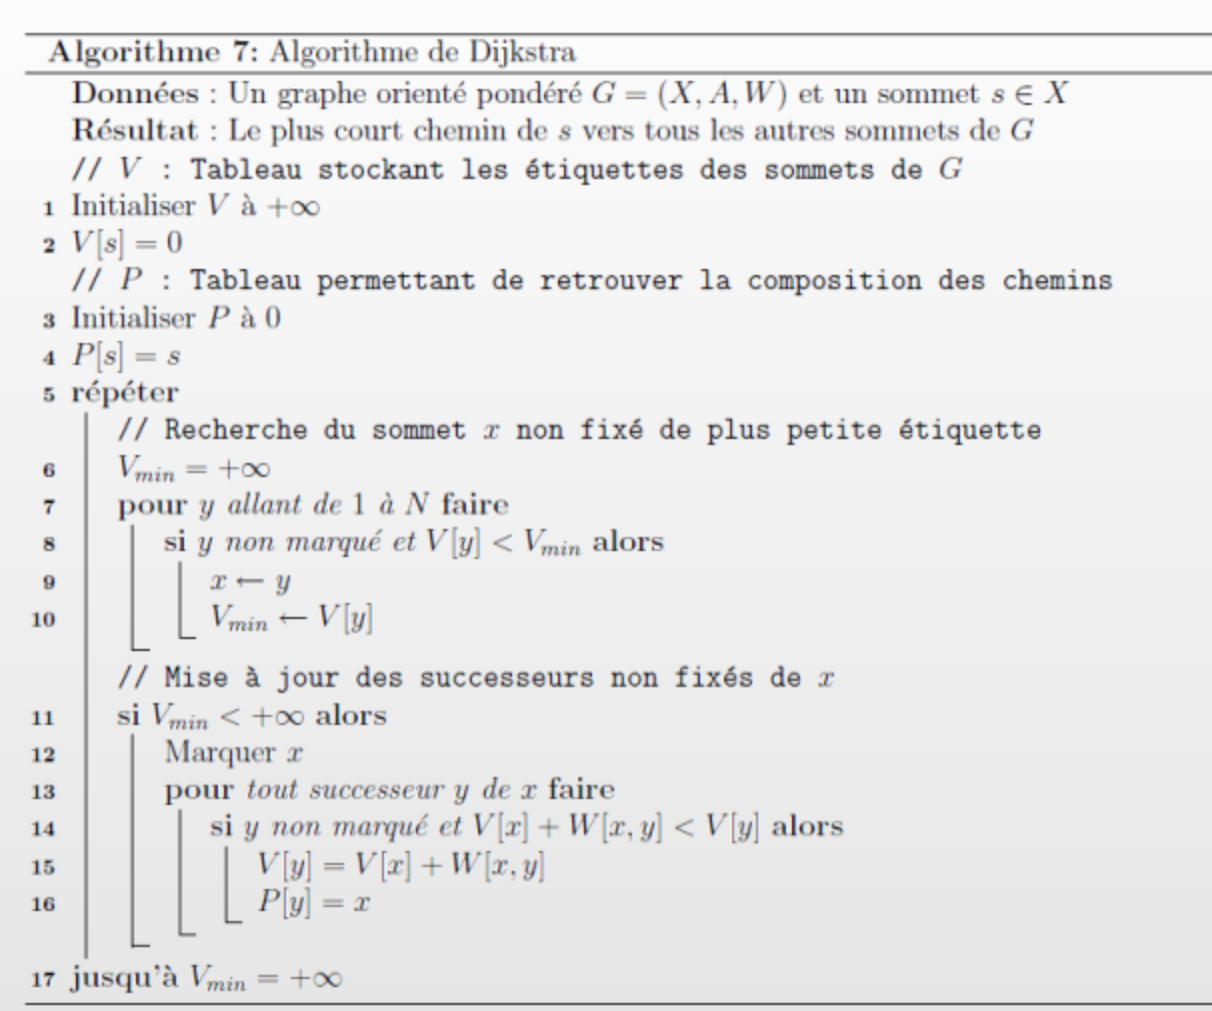
\includegraphics[scale=0.2]{dijkstra-explication.png}
On sort de Dijkstra le plus court chemin de A \'a B puis si celui ci est plein on peut r\'eappliquer ce m\^eme programme pour trouver le suivant. C'est donc fold fulkerson.

\subsubsection{}
\begin{tikzpicture}[scale=3]
	\axes{n}{v}{1}{0.6}
	\valx{0.9}{$n_{max}$}
	\valy{0.5}{$v_{max}$}
	\draw[line width = 0.3mm, color=red] (0,0.5)--(0.9,0);
\end{tikzpicture}

Ce modèle permet de représenter la décroissance de vitesse, avec l’augmentation du nombre de voitures. La vitesse initiale est $v_{max}$, et elle atteint 0 en $n_{max}$. Cependant, la vitesse décroît dès la première voiture, ce qui n’est pas très réaliste. Ce modèle permet aussi une implémentation assez simple.


\subsubsection{}
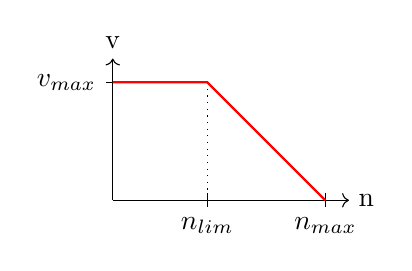
\begin{tikzpicture}[scale=3]
	\axes{n}{v}{1}{0.6}
	\valx{0.9}{$n_{max}$}
	\valx{0.4}{$n_{lim}$}
	\valy{0.5}{$v_{max}$}
	\draw[dotted] (0.4,0.5) -- (0.4,0);
	\draw[line width = 0.3mm, color=red] (0,0.5)--(0.4,0.5) -- (0.9,0);
\end{tikzpicture}

Combinaison des deux précédents, ce modèle considère une vitesse constante ($v_{max}$) jusqu’à un nombre de voitures limite ($n_{lim}$) qui déclenche une diminution de la vitesse. Celle ci décroît jusqu’à atteindre 0 pour le nombre maximum de voitures que peut atteindre la route ($n_{max}$). Ce modèle est bien plus réaliste, même si la décroissance linéaire reste très approximative.

\subsubsection{}
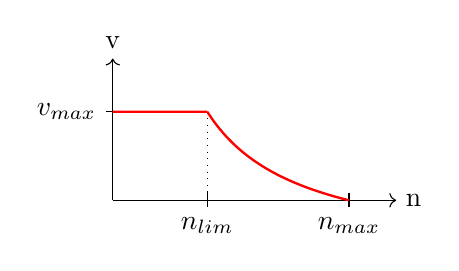
\begin{tikzpicture}[scale=3]
	\axes{n}{v}{1.2}{0.6}
	\valx{1}{$n_{max}$}
	\valx{0.4}{$n_{lim}$}
	\valy{0.375}{$v_{max}$}
	\draw[dotted] (0.4,0.375) -- (0.4,0);
	\draw[line width = 0.3mm, color=red] (0,0.375)--(0.4,0.375) [domain=0.4:1,line width=0.3mm, smooth, variable=\x, red] plot ({\x}, {(1/(4*\x)-0.25)});
\end{tikzpicture}
\newpage

\newpage
\subsection{Expression de la fonction d'évaluation}
voitures indicées $1,...,i,...N$\\
routes empruntées indicées $1,...,l,...,R$\\
chemins indicés $1,...,k,...,C$\\
temps de parcours $T_1,...,T_k,...,T_R$\\
nombre de voitures sur le chemin k $\lambda_k = \sum_{i=1}^N 
\delta_{c(i),k}$\\
avec c(i) l'indice du chemin emprunté par la voiture i\\
$\chi_{l,k} = $ 1 si la route l est dans le chemin k et 0 sinon\\
T(k) : temps de parcours du chemin k = $\sum_{l=1}^R T_l \chi_l (k)$

\newpage
\subsection{resolution par descente de gradiant}
pour ce qui est de la r\'esolution pour des fonctions de vitesse compliqu\'ees, on se ramm\`ene \`a minimiser la fonction qui a une repartition sur les diff\'erents chemins associe le temps de parcours de la plus lente des voitures.\\
Consid\'erons les chemins $c_1,\cdots,c_n$ dans un certain ordre et consid\'erons en entr\'ee de notre fonction d'\'evaluation la r\'epartition des voitures $\lambda_1,\lambda_2,\cdots,\lambda_n \in [0,1]$, avec $\sum_{i=1}^n \lambda_i = 1$. Si $\lambda_i=0.2$ on dirige 20\% des voitures sur le chemin i. 

\end{document}
